\documentclass[14pt]{extbook}
\usepackage{multicol, enumerate, enumitem, hyperref, color, soul, setspace, parskip, fancyhdr} %General Packages
\usepackage{amssymb, amsthm, amsmath, bbm, latexsym, units, mathtools} %Math Packages
\everymath{\displaystyle} %All math in Display Style
% Packages with additional options
\usepackage[headsep=0.5cm,headheight=12pt, left=1 in,right= 1 in,top= 1 in,bottom= 1 in]{geometry}
\usepackage[usenames,dvipsnames]{xcolor}
\usepackage{dashrule}  % Package to use the command below to create lines between items
\newcommand{\litem}[1]{\item#1\hspace*{-1cm}\rule{\textwidth}{0.4pt}}
\pagestyle{fancy}
\lhead{Progress Quiz 3}
\chead{}
\rhead{Version C}
\lfoot{}
\cfoot{}
\rfoot{Fall 2020}
\begin{document}

\begin{enumerate}
\litem{
Describe the end behavior of the polynomial below.\[ f(x) = -8(x + 9)^{4}(x - 9)^{5}(x - 2)^{5}(x + 2)^{6} \]\begin{enumerate}[label=\Alph*.]
\begin{multicols}{2}\item 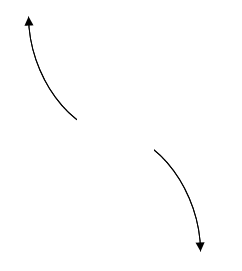
\includegraphics[width = 0.3\textwidth]{../Figures/polyEndBehaviorAC.png}\item 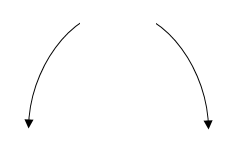
\includegraphics[width = 0.3\textwidth]{../Figures/polyEndBehaviorBC.png}\item 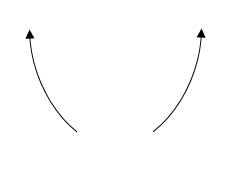
\includegraphics[width = 0.3\textwidth]{../Figures/polyEndBehaviorCC.png}\item 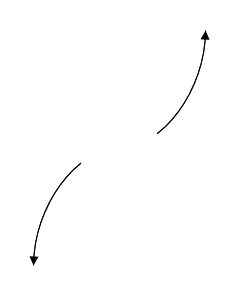
\includegraphics[width = 0.3\textwidth]{../Figures/polyEndBehaviorDC.png}\end{multicols}\item None of the above.
\end{enumerate} }
\litem{
Describe the zero behavior of the zero $x = 2$ of the polynomial below.\[ f(x) = -5(x + 8)^{9}(x - 8)^{5}(x - 2)^{6}(x + 2)^{5} \]\begin{enumerate}[label=\Alph*.]
\begin{multicols}{2}\item 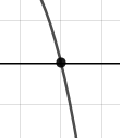
\includegraphics[width = 0.3\textwidth]{../Figures/polyZeroBehaviorAC.png}\item 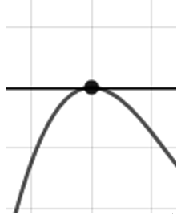
\includegraphics[width = 0.3\textwidth]{../Figures/polyZeroBehaviorBC.png}\item 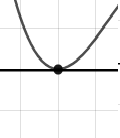
\includegraphics[width = 0.3\textwidth]{../Figures/polyZeroBehaviorCC.png}\item 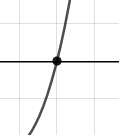
\includegraphics[width = 0.3\textwidth]{../Figures/polyZeroBehaviorDC.png}\end{multicols}\item None of the above.
\end{enumerate} }
\litem{
Which of the following equations \textit{could} be of the graph presented below?
\begin{center}
    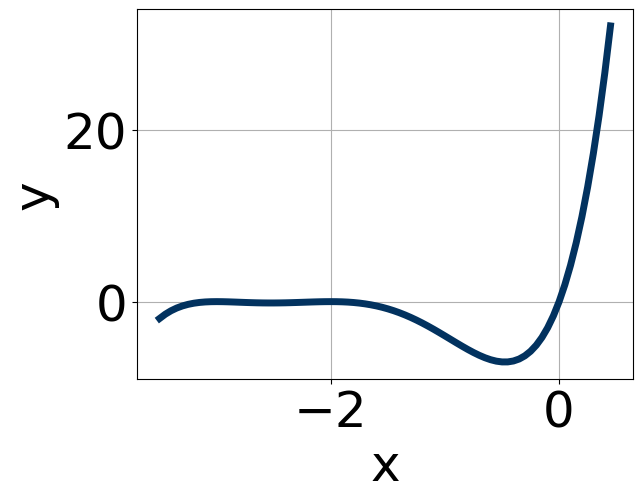
\includegraphics[width=0.5\textwidth]{../Figures/polyGraphToFunctionCopyC.png}
\end{center}
\begin{enumerate}[label=\Alph*.]
\item \( 12x^{7} (x + 3)^{10} (x + 2)^{4} \)
\item \( 14x^{8} (x + 3)^{6} (x + 2)^{5} \)
\item \( -5x^{6} (x + 3)^{4} (x + 2)^{6} \)
\item \( 15x^{5} (x + 3)^{6} (x + 2)^{7} \)
\item \( -17x^{5} (x + 3)^{6} (x + 2)^{6} \)

\end{enumerate} }
\litem{
Describe the end behavior of the polynomial below.\[ f(x) = -3(x - 5)^{4}(x + 5)^{5}(x + 9)^{3}(x - 9)^{4} \]\begin{enumerate}[label=\Alph*.]
\begin{multicols}{2}\item 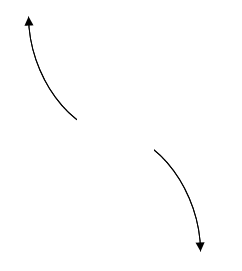
\includegraphics[width = 0.3\textwidth]{../Figures/polyEndBehaviorCopyAC.png}\item 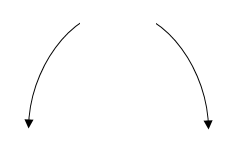
\includegraphics[width = 0.3\textwidth]{../Figures/polyEndBehaviorCopyBC.png}\item 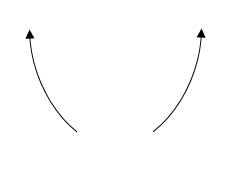
\includegraphics[width = 0.3\textwidth]{../Figures/polyEndBehaviorCopyCC.png}\item 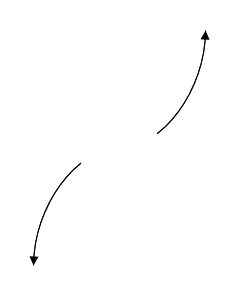
\includegraphics[width = 0.3\textwidth]{../Figures/polyEndBehaviorCopyDC.png}\end{multicols}\item None of the above.
\end{enumerate} }
\litem{
Construct the lowest-degree polynomial given the zeros below. Then, choose the intervals that contain the coefficients of the polynomial in the form $x^3+bx^2+cx+d$.\[ -5 + 2 i \text{ and } -2 \]\begin{enumerate}[label=\Alph*.]
\item \( b \in [0, 3], c \in [-4, 3], \text{ and } d \in [-7, -1] \)
\item \( b \in [11, 17], c \in [48, 50], \text{ and } d \in [57, 61] \)
\item \( b \in [0, 3], c \in [4, 10], \text{ and } d \in [3, 13] \)
\item \( b \in [-13, -10], c \in [48, 50], \text{ and } d \in [-61, -53] \)
\item \( \text{None of the above.} \)

\end{enumerate} }
\litem{
Construct the lowest-degree polynomial given the zeros below. Then, choose the intervals that contain the coefficients of the polynomial in the form $ax^3+bx^2+cx+d$.\[ \frac{1}{3}, \frac{2}{5}, \text{ and } \frac{1}{2} \]\begin{enumerate}[label=\Alph*.]
\item \( a \in [29, 32], b \in [36, 40], c \in [10, 16], \text{ and } d \in [0.7, 3.2] \)
\item \( a \in [29, 32], b \in [1, 12], c \in [-11, -6], \text{ and } d \in [-2.2, -0.1] \)
\item \( a \in [29, 32], b \in [-40, -33], c \in [10, 16], \text{ and } d \in [0.7, 3.2] \)
\item \( a \in [29, 32], b \in [-21, -15], c \in [-3, 0], \text{ and } d \in [0.7, 3.2] \)
\item \( a \in [29, 32], b \in [-40, -33], c \in [10, 16], \text{ and } d \in [-2.2, -0.1] \)

\end{enumerate} }
\litem{
Construct the lowest-degree polynomial given the zeros below. Then, choose the intervals that contain the coefficients of the polynomial in the form $ax^3+bx^2+cx+d$.\[ \frac{2}{5}, \frac{-7}{5}, \text{ and } 3 \]\begin{enumerate}[label=\Alph*.]
\item \( a \in [22, 30], b \in [-53, -44], c \in [-89, -85], \text{ and } d \in [32, 48] \)
\item \( a \in [22, 30], b \in [-53, -44], c \in [-89, -85], \text{ and } d \in [-44, -39] \)
\item \( a \in [22, 30], b \in [-30, -29], c \in [-128, -119], \text{ and } d \in [-44, -39] \)
\item \( a \in [22, 30], b \in [50, 51], c \in [-89, -85], \text{ and } d \in [-44, -39] \)
\item \( a \in [22, 30], b \in [-108, -96], c \in [60, 64], \text{ and } d \in [32, 48] \)

\end{enumerate} }
\litem{
Construct the lowest-degree polynomial given the zeros below. Then, choose the intervals that contain the coefficients of the polynomial in the form $x^3+bx^2+cx+d$.\[ -3 + 2 i \text{ and } -3 \]\begin{enumerate}[label=\Alph*.]
\item \( b \in [-2, 6], c \in [2, 11], \text{ and } d \in [7, 14] \)
\item \( b \in [-2, 6], c \in [1, 2], \text{ and } d \in [-12, 2] \)
\item \( b \in [5, 21], c \in [23, 38], \text{ and } d \in [39, 45] \)
\item \( b \in [-10, -8], c \in [23, 38], \text{ and } d \in [-40, -33] \)
\item \( \text{None of the above.} \)

\end{enumerate} }
\litem{
Describe the zero behavior of the zero $x = 8$ of the polynomial below.\[ f(x) = 2(x + 3)^{13}(x - 3)^{9}(x + 8)^{12}(x - 8)^{7} \]\begin{enumerate}[label=\Alph*.]
\begin{multicols}{2}\item 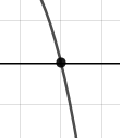
\includegraphics[width = 0.3\textwidth]{../Figures/polyZeroBehaviorCopyAC.png}\item 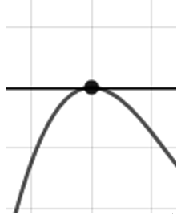
\includegraphics[width = 0.3\textwidth]{../Figures/polyZeroBehaviorCopyBC.png}\item 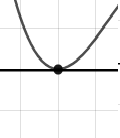
\includegraphics[width = 0.3\textwidth]{../Figures/polyZeroBehaviorCopyCC.png}\item 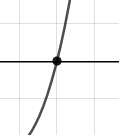
\includegraphics[width = 0.3\textwidth]{../Figures/polyZeroBehaviorCopyDC.png}\end{multicols}\item None of the above.
\end{enumerate} }
\litem{
Which of the following equations \textit{could} be of the graph presented below?
\begin{center}
    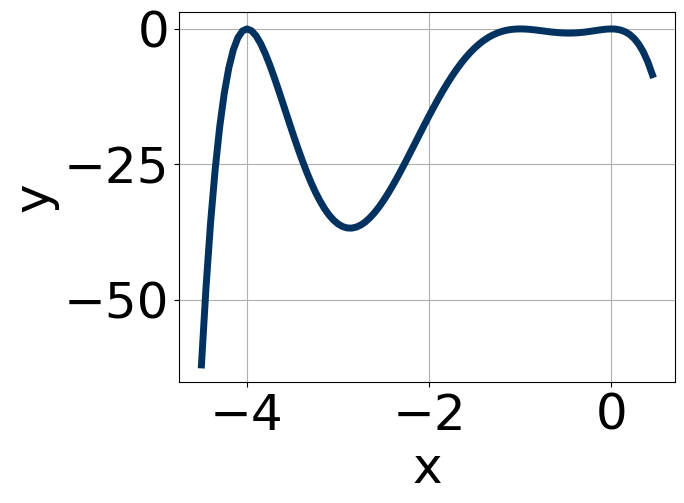
\includegraphics[width=0.5\textwidth]{../Figures/polyGraphToFunctionC.png}
\end{center}
\begin{enumerate}[label=\Alph*.]
\item \( 19x^{10} (x + 4)^{4} (x + 1)^{5} \)
\item \( -19x^{4} (x + 4)^{6} (x + 1)^{4} \)
\item \( -18x^{8} (x + 4)^{10} (x + 1)^{11} \)
\item \( -11x^{7} (x + 4)^{6} (x + 1)^{5} \)
\item \( 4x^{4} (x + 4)^{8} (x + 1)^{10} \)

\end{enumerate} }
\end{enumerate}

\end{document}